\documentclass[twoside]{book}

% Packages required by doxygen
\usepackage{fixltx2e}
\usepackage{calc}
\usepackage{doxygen}
\usepackage[export]{adjustbox} % also loads graphicx
\usepackage{graphicx}
\usepackage[utf8]{inputenc}
\usepackage{makeidx}
\usepackage{multicol}
\usepackage{multirow}
\PassOptionsToPackage{warn}{textcomp}
\usepackage{textcomp}
\usepackage[nointegrals]{wasysym}
\usepackage[table]{xcolor}

% Font selection
\usepackage[T1]{fontenc}
\usepackage[scaled=.90]{helvet}
\usepackage{courier}
\usepackage{amssymb}
\usepackage{sectsty}
\renewcommand{\familydefault}{\sfdefault}
\allsectionsfont{%
  \fontseries{bc}\selectfont%
  \color{darkgray}%
}
\renewcommand{\DoxyLabelFont}{%
  \fontseries{bc}\selectfont%
  \color{darkgray}%
}
\newcommand{\+}{\discretionary{\mbox{\scriptsize$\hookleftarrow$}}{}{}}

% Page & text layout
\usepackage{geometry}
\geometry{%
  a4paper,%
  top=2.5cm,%
  bottom=2.5cm,%
  left=2.5cm,%
  right=2.5cm%
}
\tolerance=750
\hfuzz=15pt
\hbadness=750
\setlength{\emergencystretch}{15pt}
\setlength{\parindent}{0cm}
\setlength{\parskip}{3ex plus 2ex minus 2ex}
\makeatletter
\renewcommand{\paragraph}{%
  \@startsection{paragraph}{4}{0ex}{-1.0ex}{1.0ex}{%
    \normalfont\normalsize\bfseries\SS@parafont%
  }%
}
\renewcommand{\subparagraph}{%
  \@startsection{subparagraph}{5}{0ex}{-1.0ex}{1.0ex}{%
    \normalfont\normalsize\bfseries\SS@subparafont%
  }%
}
\makeatother

% Headers & footers
\usepackage{fancyhdr}
\pagestyle{fancyplain}
\fancyhead[LE]{\fancyplain{}{\bfseries\thepage}}
\fancyhead[CE]{\fancyplain{}{}}
\fancyhead[RE]{\fancyplain{}{\bfseries\leftmark}}
\fancyhead[LO]{\fancyplain{}{\bfseries\rightmark}}
\fancyhead[CO]{\fancyplain{}{}}
\fancyhead[RO]{\fancyplain{}{\bfseries\thepage}}
\fancyfoot[LE]{\fancyplain{}{}}
\fancyfoot[CE]{\fancyplain{}{}}
\fancyfoot[RE]{\fancyplain{}{\bfseries\scriptsize Generated by Doxygen }}
\fancyfoot[LO]{\fancyplain{}{\bfseries\scriptsize Generated by Doxygen }}
\fancyfoot[CO]{\fancyplain{}{}}
\fancyfoot[RO]{\fancyplain{}{}}
\renewcommand{\footrulewidth}{0.4pt}
\renewcommand{\chaptermark}[1]{%
  \markboth{#1}{}%
}
\renewcommand{\sectionmark}[1]{%
  \markright{\thesection\ #1}%
}

% Indices & bibliography
\usepackage{natbib}
\usepackage[titles]{tocloft}
\setcounter{tocdepth}{3}
\setcounter{secnumdepth}{5}
\makeindex

% Hyperlinks (required, but should be loaded last)
\usepackage{ifpdf}
\ifpdf
  \usepackage[pdftex,pagebackref=true]{hyperref}
\else
  \usepackage[ps2pdf,pagebackref=true]{hyperref}
\fi
\hypersetup{%
  colorlinks=true,%
  linkcolor=blue,%
  citecolor=blue,%
  unicode%
}

% Custom commands
\newcommand{\clearemptydoublepage}{%
  \newpage{\pagestyle{empty}\cleardoublepage}%
}

\usepackage{caption}
\captionsetup{labelsep=space,justification=centering,font={bf},singlelinecheck=off,skip=4pt,position=top}

%===== C O N T E N T S =====

\begin{document}

% Titlepage & ToC
\hypersetup{pageanchor=false,
             bookmarksnumbered=true,
             pdfencoding=unicode
            }
\pagenumbering{alph}
\begin{titlepage}
\vspace*{7cm}
\begin{center}%
{\Large tsp-\/framework }\\
\vspace*{1cm}
{\large Generated by Doxygen 1.8.14}\\
\end{center}
\end{titlepage}
\clearemptydoublepage
\pagenumbering{roman}
\tableofcontents
\clearemptydoublepage
\pagenumbering{arabic}
\hypersetup{pageanchor=true}

%--- Begin generated contents ---
\chapter{Hierarchical Index}
\section{Class Hierarchy}
This inheritance list is sorted roughly, but not completely, alphabetically\+:\begin{DoxyCompactList}
\item \contentsline{section}{tsp.\+heuristic.\+A\+Heuristic}{\pageref{classtsp_1_1heuristic_1_1_a_heuristic}}{}
\item \contentsline{section}{tsp.\+metaheuristic.\+A\+Metaheuristic}{\pageref{classtsp_1_1metaheuristic_1_1_a_metaheuristic}}{}
\item \contentsline{section}{tsp.\+neighborhood.\+A\+Neighborhood}{\pageref{classtsp_1_1neighborhood_1_1_a_neighborhood}}{}
\item \contentsline{section}{tsp.\+Instance}{\pageref{classtsp_1_1_instance}}{}
\item \contentsline{section}{tsp.\+Main}{\pageref{classtsp_1_1_main}}{}
\item \contentsline{section}{tsp.\+Solution}{\pageref{classtsp_1_1_solution}}{}
\item \contentsline{section}{tsp.\+T\+S\+P\+Solver}{\pageref{classtsp_1_1_t_s_p_solver}}{}
\item Action\+Listener\begin{DoxyCompactList}
\item \contentsline{section}{tsp.\+gui.\+T\+S\+P\+G\+UI}{\pageref{classtsp_1_1gui_1_1_t_s_p_g_u_i}}{}
\end{DoxyCompactList}
\item J\+Frame\begin{DoxyCompactList}
\item \contentsline{section}{tsp.\+gui.\+T\+S\+P\+G\+UI}{\pageref{classtsp_1_1gui_1_1_t_s_p_g_u_i}}{}
\end{DoxyCompactList}
\end{DoxyCompactList}

\chapter{Class Index}
\section{Class List}
Here are the classes, structs, unions and interfaces with brief descriptions\+:\begin{DoxyCompactList}
\item\contentsline{section}{\mbox{\hyperlink{classtsp_1_1heuristic_1_1_a_heuristic}{tsp.\+heuristic.\+A\+Heuristic}} }{\pageref{classtsp_1_1heuristic_1_1_a_heuristic}}{}
\item\contentsline{section}{\mbox{\hyperlink{classtsp_1_1metaheuristic_1_1_a_metaheuristic}{tsp.\+metaheuristic.\+A\+Metaheuristic}} }{\pageref{classtsp_1_1metaheuristic_1_1_a_metaheuristic}}{}
\item\contentsline{section}{\mbox{\hyperlink{classtsp_1_1neighborhood_1_1_a_neighborhood}{tsp.\+neighborhood.\+A\+Neighborhood}} }{\pageref{classtsp_1_1neighborhood_1_1_a_neighborhood}}{}
\item\contentsline{section}{\mbox{\hyperlink{classtsp_1_1_instance}{tsp.\+Instance}} }{\pageref{classtsp_1_1_instance}}{}
\item\contentsline{section}{\mbox{\hyperlink{classtsp_1_1_main}{tsp.\+Main}} }{\pageref{classtsp_1_1_main}}{}
\item\contentsline{section}{\mbox{\hyperlink{classtsp_1_1_solution}{tsp.\+Solution}} }{\pageref{classtsp_1_1_solution}}{}
\item\contentsline{section}{\mbox{\hyperlink{classtsp_1_1gui_1_1_t_s_p_g_u_i}{tsp.\+gui.\+T\+S\+P\+G\+UI}} }{\pageref{classtsp_1_1gui_1_1_t_s_p_g_u_i}}{}
\item\contentsline{section}{\mbox{\hyperlink{classtsp_1_1_t_s_p_solver}{tsp.\+T\+S\+P\+Solver}} }{\pageref{classtsp_1_1_t_s_p_solver}}{}
\end{DoxyCompactList}

\chapter{Class Documentation}
\hypertarget{classtsp_1_1heuristic_1_1_a_heuristic}{}\section{tsp.\+heuristic.\+A\+Heuristic Class Reference}
\label{classtsp_1_1heuristic_1_1_a_heuristic}\index{tsp.\+heuristic.\+A\+Heuristic@{tsp.\+heuristic.\+A\+Heuristic}}
\subsection*{Public Member Functions}
\begin{DoxyCompactItemize}
\item 
\mbox{\hyperlink{classtsp_1_1heuristic_1_1_a_heuristic_a7eacbf5e1305f1cdedc1fd2b9765f766}{A\+Heuristic}} (\mbox{\hyperlink{classtsp_1_1_instance}{Instance}} instance, String name)  throws Exception 
\item 
abstract \mbox{\hyperlink{classtsp_1_1_solution}{Solution}} \mbox{\hyperlink{classtsp_1_1heuristic_1_1_a_heuristic_a4aba2cc94bfc0e00d2b70c5dbdd8b944}{solve}} ()  throws Exception
\item 
\mbox{\hyperlink{classtsp_1_1_solution}{Solution}} \mbox{\hyperlink{classtsp_1_1heuristic_1_1_a_heuristic_a4a30417f030073fefcd1f1306aaaec51}{get\+Solution}} ()
\item 
String \mbox{\hyperlink{classtsp_1_1heuristic_1_1_a_heuristic_a8757a9661d1a3ca486cf8ceaa80d240a}{get\+Name}} ()
\end{DoxyCompactItemize}
\subsection*{Protected Attributes}
\begin{DoxyCompactItemize}
\item 
\mbox{\hyperlink{classtsp_1_1_instance}{Instance}} \mbox{\hyperlink{classtsp_1_1heuristic_1_1_a_heuristic_a8be1dd6cd9c5a8cd8ed839d46c7cb85f}{m\+\_\+instance}}
\item 
\mbox{\hyperlink{classtsp_1_1_solution}{Solution}} \mbox{\hyperlink{classtsp_1_1heuristic_1_1_a_heuristic_a43dda539b2ed7ca67172c97951a2bde9}{m\+\_\+solution}}
\item 
String \mbox{\hyperlink{classtsp_1_1heuristic_1_1_a_heuristic_a909754c0caf21979fa1d3c8bee42c000}{m\+\_\+name}}
\end{DoxyCompactItemize}


\subsection{Detailed Description}
This is the abstract class for Heuristic \begin{DoxyAuthor}{Author}
Axel Grimault 
\end{DoxyAuthor}
\begin{DoxyVersion}{Version}
2017 
\end{DoxyVersion}


\subsection{Constructor \& Destructor Documentation}
\mbox{\Hypertarget{classtsp_1_1heuristic_1_1_a_heuristic_a7eacbf5e1305f1cdedc1fd2b9765f766}\label{classtsp_1_1heuristic_1_1_a_heuristic_a7eacbf5e1305f1cdedc1fd2b9765f766}} 
\index{tsp\+::heuristic\+::\+A\+Heuristic@{tsp\+::heuristic\+::\+A\+Heuristic}!A\+Heuristic@{A\+Heuristic}}
\index{A\+Heuristic@{A\+Heuristic}!tsp\+::heuristic\+::\+A\+Heuristic@{tsp\+::heuristic\+::\+A\+Heuristic}}
\subsubsection{\texorpdfstring{A\+Heuristic()}{AHeuristic()}}
{\footnotesize\ttfamily tsp.\+heuristic.\+A\+Heuristic.\+A\+Heuristic (\begin{DoxyParamCaption}\item[{\mbox{\hyperlink{classtsp_1_1_instance}{Instance}}}]{instance,  }\item[{String}]{name }\end{DoxyParamCaption}) throws Exception\hspace{0.3cm}{\ttfamily [inline]}}

Constructor 
\begin{DoxyParams}{Parameters}
{\em instance} & the instance of the problem \\
\hline
{\em name} & the name of the metaheuristic \\
\hline
\end{DoxyParams}


\subsection{Member Function Documentation}
\mbox{\Hypertarget{classtsp_1_1heuristic_1_1_a_heuristic_a8757a9661d1a3ca486cf8ceaa80d240a}\label{classtsp_1_1heuristic_1_1_a_heuristic_a8757a9661d1a3ca486cf8ceaa80d240a}} 
\index{tsp\+::heuristic\+::\+A\+Heuristic@{tsp\+::heuristic\+::\+A\+Heuristic}!get\+Name@{get\+Name}}
\index{get\+Name@{get\+Name}!tsp\+::heuristic\+::\+A\+Heuristic@{tsp\+::heuristic\+::\+A\+Heuristic}}
\subsubsection{\texorpdfstring{get\+Name()}{getName()}}
{\footnotesize\ttfamily String tsp.\+heuristic.\+A\+Heuristic.\+get\+Name (\begin{DoxyParamCaption}{ }\end{DoxyParamCaption})\hspace{0.3cm}{\ttfamily [inline]}}

Returns the name of the heuristic \mbox{\Hypertarget{classtsp_1_1heuristic_1_1_a_heuristic_a4a30417f030073fefcd1f1306aaaec51}\label{classtsp_1_1heuristic_1_1_a_heuristic_a4a30417f030073fefcd1f1306aaaec51}} 
\index{tsp\+::heuristic\+::\+A\+Heuristic@{tsp\+::heuristic\+::\+A\+Heuristic}!get\+Solution@{get\+Solution}}
\index{get\+Solution@{get\+Solution}!tsp\+::heuristic\+::\+A\+Heuristic@{tsp\+::heuristic\+::\+A\+Heuristic}}
\subsubsection{\texorpdfstring{get\+Solution()}{getSolution()}}
{\footnotesize\ttfamily \mbox{\hyperlink{classtsp_1_1_solution}{Solution}} tsp.\+heuristic.\+A\+Heuristic.\+get\+Solution (\begin{DoxyParamCaption}{ }\end{DoxyParamCaption})\hspace{0.3cm}{\ttfamily [inline]}}

Returns the solution built with this heuristic \mbox{\Hypertarget{classtsp_1_1heuristic_1_1_a_heuristic_a4aba2cc94bfc0e00d2b70c5dbdd8b944}\label{classtsp_1_1heuristic_1_1_a_heuristic_a4aba2cc94bfc0e00d2b70c5dbdd8b944}} 
\index{tsp\+::heuristic\+::\+A\+Heuristic@{tsp\+::heuristic\+::\+A\+Heuristic}!solve@{solve}}
\index{solve@{solve}!tsp\+::heuristic\+::\+A\+Heuristic@{tsp\+::heuristic\+::\+A\+Heuristic}}
\subsubsection{\texorpdfstring{solve()}{solve()}}
{\footnotesize\ttfamily abstract \mbox{\hyperlink{classtsp_1_1_solution}{Solution}} tsp.\+heuristic.\+A\+Heuristic.\+solve (\begin{DoxyParamCaption}{ }\end{DoxyParamCaption}) throws Exception\hspace{0.3cm}{\ttfamily [abstract]}}

Apply the heuristic to build m\+\_\+solution 

\subsection{Member Data Documentation}
\mbox{\Hypertarget{classtsp_1_1heuristic_1_1_a_heuristic_a8be1dd6cd9c5a8cd8ed839d46c7cb85f}\label{classtsp_1_1heuristic_1_1_a_heuristic_a8be1dd6cd9c5a8cd8ed839d46c7cb85f}} 
\index{tsp\+::heuristic\+::\+A\+Heuristic@{tsp\+::heuristic\+::\+A\+Heuristic}!m\+\_\+instance@{m\+\_\+instance}}
\index{m\+\_\+instance@{m\+\_\+instance}!tsp\+::heuristic\+::\+A\+Heuristic@{tsp\+::heuristic\+::\+A\+Heuristic}}
\subsubsection{\texorpdfstring{m\+\_\+instance}{m\_instance}}
{\footnotesize\ttfamily \mbox{\hyperlink{classtsp_1_1_instance}{Instance}} tsp.\+heuristic.\+A\+Heuristic.\+m\+\_\+instance\hspace{0.3cm}{\ttfamily [protected]}}

The data of the problem \mbox{\Hypertarget{classtsp_1_1heuristic_1_1_a_heuristic_a909754c0caf21979fa1d3c8bee42c000}\label{classtsp_1_1heuristic_1_1_a_heuristic_a909754c0caf21979fa1d3c8bee42c000}} 
\index{tsp\+::heuristic\+::\+A\+Heuristic@{tsp\+::heuristic\+::\+A\+Heuristic}!m\+\_\+name@{m\+\_\+name}}
\index{m\+\_\+name@{m\+\_\+name}!tsp\+::heuristic\+::\+A\+Heuristic@{tsp\+::heuristic\+::\+A\+Heuristic}}
\subsubsection{\texorpdfstring{m\+\_\+name}{m\_name}}
{\footnotesize\ttfamily String tsp.\+heuristic.\+A\+Heuristic.\+m\+\_\+name\hspace{0.3cm}{\ttfamily [protected]}}

The name of the heuristic \mbox{\Hypertarget{classtsp_1_1heuristic_1_1_a_heuristic_a43dda539b2ed7ca67172c97951a2bde9}\label{classtsp_1_1heuristic_1_1_a_heuristic_a43dda539b2ed7ca67172c97951a2bde9}} 
\index{tsp\+::heuristic\+::\+A\+Heuristic@{tsp\+::heuristic\+::\+A\+Heuristic}!m\+\_\+solution@{m\+\_\+solution}}
\index{m\+\_\+solution@{m\+\_\+solution}!tsp\+::heuristic\+::\+A\+Heuristic@{tsp\+::heuristic\+::\+A\+Heuristic}}
\subsubsection{\texorpdfstring{m\+\_\+solution}{m\_solution}}
{\footnotesize\ttfamily \mbox{\hyperlink{classtsp_1_1_solution}{Solution}} tsp.\+heuristic.\+A\+Heuristic.\+m\+\_\+solution\hspace{0.3cm}{\ttfamily [protected]}}

The solution built 

The documentation for this class was generated from the following file\+:\begin{DoxyCompactItemize}
\item 
src/tsp/heuristic/A\+Heuristic.\+java\end{DoxyCompactItemize}

\hypertarget{classtsp_1_1metaheuristic_1_1_a_metaheuristic}{}\section{tsp.\+metaheuristic.\+A\+Metaheuristic Class Reference}
\label{classtsp_1_1metaheuristic_1_1_a_metaheuristic}\index{tsp.\+metaheuristic.\+A\+Metaheuristic@{tsp.\+metaheuristic.\+A\+Metaheuristic}}
\subsection*{Public Member Functions}
\begin{DoxyCompactItemize}
\item 
\mbox{\hyperlink{classtsp_1_1metaheuristic_1_1_a_metaheuristic_a8a5f85f47ae51d4e389c3335f5c32350}{A\+Metaheuristic}} (\mbox{\hyperlink{classtsp_1_1_instance}{Instance}} instance, String name)  throws Exception 
\item 
abstract \mbox{\hyperlink{classtsp_1_1_solution}{Solution}} \mbox{\hyperlink{classtsp_1_1metaheuristic_1_1_a_metaheuristic_a0bff8acfcbdb9170d9d6090d3b66efff}{solve}} (\mbox{\hyperlink{classtsp_1_1_solution}{Solution}} sol)  throws Exception
\item 
String \mbox{\hyperlink{classtsp_1_1metaheuristic_1_1_a_metaheuristic_af6a576aa8c6e48ebd22ea5d02cf7e1d6}{get\+Name}} ()
\end{DoxyCompactItemize}
\subsection*{Protected Attributes}
\begin{DoxyCompactItemize}
\item 
\mbox{\hyperlink{classtsp_1_1_instance}{Instance}} \mbox{\hyperlink{classtsp_1_1metaheuristic_1_1_a_metaheuristic_aa25dbfb4c96866bce856787dd30352b5}{m\+\_\+instance}}
\item 
String \mbox{\hyperlink{classtsp_1_1metaheuristic_1_1_a_metaheuristic_a9e4b4a3b7555598bf92d825ada066a75}{m\+\_\+name}}
\end{DoxyCompactItemize}


\subsection{Detailed Description}
This is the abstract class for Metaheuristic \begin{DoxyAuthor}{Author}
Axel Grimault 
\end{DoxyAuthor}
\begin{DoxyVersion}{Version}
2017 
\end{DoxyVersion}


\subsection{Constructor \& Destructor Documentation}
\mbox{\Hypertarget{classtsp_1_1metaheuristic_1_1_a_metaheuristic_a8a5f85f47ae51d4e389c3335f5c32350}\label{classtsp_1_1metaheuristic_1_1_a_metaheuristic_a8a5f85f47ae51d4e389c3335f5c32350}} 
\index{tsp\+::metaheuristic\+::\+A\+Metaheuristic@{tsp\+::metaheuristic\+::\+A\+Metaheuristic}!A\+Metaheuristic@{A\+Metaheuristic}}
\index{A\+Metaheuristic@{A\+Metaheuristic}!tsp\+::metaheuristic\+::\+A\+Metaheuristic@{tsp\+::metaheuristic\+::\+A\+Metaheuristic}}
\subsubsection{\texorpdfstring{A\+Metaheuristic()}{AMetaheuristic()}}
{\footnotesize\ttfamily tsp.\+metaheuristic.\+A\+Metaheuristic.\+A\+Metaheuristic (\begin{DoxyParamCaption}\item[{\mbox{\hyperlink{classtsp_1_1_instance}{Instance}}}]{instance,  }\item[{String}]{name }\end{DoxyParamCaption}) throws Exception\hspace{0.3cm}{\ttfamily [inline]}}

Constructor 
\begin{DoxyParams}{Parameters}
{\em instance} & the instance of the problem \\
\hline
{\em name} & the name of the metaheuristic \\
\hline
\end{DoxyParams}


\subsection{Member Function Documentation}
\mbox{\Hypertarget{classtsp_1_1metaheuristic_1_1_a_metaheuristic_af6a576aa8c6e48ebd22ea5d02cf7e1d6}\label{classtsp_1_1metaheuristic_1_1_a_metaheuristic_af6a576aa8c6e48ebd22ea5d02cf7e1d6}} 
\index{tsp\+::metaheuristic\+::\+A\+Metaheuristic@{tsp\+::metaheuristic\+::\+A\+Metaheuristic}!get\+Name@{get\+Name}}
\index{get\+Name@{get\+Name}!tsp\+::metaheuristic\+::\+A\+Metaheuristic@{tsp\+::metaheuristic\+::\+A\+Metaheuristic}}
\subsubsection{\texorpdfstring{get\+Name()}{getName()}}
{\footnotesize\ttfamily String tsp.\+metaheuristic.\+A\+Metaheuristic.\+get\+Name (\begin{DoxyParamCaption}{ }\end{DoxyParamCaption})\hspace{0.3cm}{\ttfamily [inline]}}

Get the name of the metaheuristic \mbox{\Hypertarget{classtsp_1_1metaheuristic_1_1_a_metaheuristic_a0bff8acfcbdb9170d9d6090d3b66efff}\label{classtsp_1_1metaheuristic_1_1_a_metaheuristic_a0bff8acfcbdb9170d9d6090d3b66efff}} 
\index{tsp\+::metaheuristic\+::\+A\+Metaheuristic@{tsp\+::metaheuristic\+::\+A\+Metaheuristic}!solve@{solve}}
\index{solve@{solve}!tsp\+::metaheuristic\+::\+A\+Metaheuristic@{tsp\+::metaheuristic\+::\+A\+Metaheuristic}}
\subsubsection{\texorpdfstring{solve()}{solve()}}
{\footnotesize\ttfamily abstract \mbox{\hyperlink{classtsp_1_1_solution}{Solution}} tsp.\+metaheuristic.\+A\+Metaheuristic.\+solve (\begin{DoxyParamCaption}\item[{\mbox{\hyperlink{classtsp_1_1_solution}{Solution}}}]{sol }\end{DoxyParamCaption}) throws Exception\hspace{0.3cm}{\ttfamily [abstract]}}

Apply the metaheuristic on a solution to get a local optimum solution 

\subsection{Member Data Documentation}
\mbox{\Hypertarget{classtsp_1_1metaheuristic_1_1_a_metaheuristic_aa25dbfb4c96866bce856787dd30352b5}\label{classtsp_1_1metaheuristic_1_1_a_metaheuristic_aa25dbfb4c96866bce856787dd30352b5}} 
\index{tsp\+::metaheuristic\+::\+A\+Metaheuristic@{tsp\+::metaheuristic\+::\+A\+Metaheuristic}!m\+\_\+instance@{m\+\_\+instance}}
\index{m\+\_\+instance@{m\+\_\+instance}!tsp\+::metaheuristic\+::\+A\+Metaheuristic@{tsp\+::metaheuristic\+::\+A\+Metaheuristic}}
\subsubsection{\texorpdfstring{m\+\_\+instance}{m\_instance}}
{\footnotesize\ttfamily \mbox{\hyperlink{classtsp_1_1_instance}{Instance}} tsp.\+metaheuristic.\+A\+Metaheuristic.\+m\+\_\+instance\hspace{0.3cm}{\ttfamily [protected]}}

The data of the problem \mbox{\Hypertarget{classtsp_1_1metaheuristic_1_1_a_metaheuristic_a9e4b4a3b7555598bf92d825ada066a75}\label{classtsp_1_1metaheuristic_1_1_a_metaheuristic_a9e4b4a3b7555598bf92d825ada066a75}} 
\index{tsp\+::metaheuristic\+::\+A\+Metaheuristic@{tsp\+::metaheuristic\+::\+A\+Metaheuristic}!m\+\_\+name@{m\+\_\+name}}
\index{m\+\_\+name@{m\+\_\+name}!tsp\+::metaheuristic\+::\+A\+Metaheuristic@{tsp\+::metaheuristic\+::\+A\+Metaheuristic}}
\subsubsection{\texorpdfstring{m\+\_\+name}{m\_name}}
{\footnotesize\ttfamily String tsp.\+metaheuristic.\+A\+Metaheuristic.\+m\+\_\+name\hspace{0.3cm}{\ttfamily [protected]}}

The name of the metaheuristic 

The documentation for this class was generated from the following file\+:\begin{DoxyCompactItemize}
\item 
src/tsp/metaheuristic/A\+Metaheuristic.\+java\end{DoxyCompactItemize}

\hypertarget{classtsp_1_1neighborhood_1_1_a_neighborhood}{}\section{tsp.\+neighborhood.\+A\+Neighborhood Class Reference}
\label{classtsp_1_1neighborhood_1_1_a_neighborhood}\index{tsp.\+neighborhood.\+A\+Neighborhood@{tsp.\+neighborhood.\+A\+Neighborhood}}
\subsection*{Public Member Functions}
\begin{DoxyCompactItemize}
\item 
\mbox{\hyperlink{classtsp_1_1neighborhood_1_1_a_neighborhood_aec2c19f05baf76258fd83483b8637da2}{A\+Neighborhood}} (\mbox{\hyperlink{classtsp_1_1_instance}{Instance}} instance, String name)  throws Exception 
\item 
abstract List$<$ \mbox{\hyperlink{classtsp_1_1_solution}{Solution}} $>$ \mbox{\hyperlink{classtsp_1_1neighborhood_1_1_a_neighborhood_a5b8c16fd20fb089c86c831e6a884b8f3}{get\+Neighborhood}} (\mbox{\hyperlink{classtsp_1_1_solution}{Solution}} sol)  throws Exception 
\item 
String \mbox{\hyperlink{classtsp_1_1neighborhood_1_1_a_neighborhood_a87ac72c2bdfadde28119eb996f92544e}{get\+Name}} ()
\end{DoxyCompactItemize}
\subsection*{Protected Attributes}
\begin{DoxyCompactItemize}
\item 
\mbox{\hyperlink{classtsp_1_1_instance}{Instance}} \mbox{\hyperlink{classtsp_1_1neighborhood_1_1_a_neighborhood_a6429b45bcc40a067c68f677a4754be9c}{m\+\_\+instance}}
\item 
String \mbox{\hyperlink{classtsp_1_1neighborhood_1_1_a_neighborhood_a8b6fb5f32e75265e1fd670a8158066b5}{m\+\_\+name}}
\end{DoxyCompactItemize}


\subsection{Detailed Description}
This is the abstract class for Neighborhood \begin{DoxyAuthor}{Author}
Axel Grimault 
\end{DoxyAuthor}
\begin{DoxyVersion}{Version}
2017 
\end{DoxyVersion}


\subsection{Constructor \& Destructor Documentation}
\mbox{\Hypertarget{classtsp_1_1neighborhood_1_1_a_neighborhood_aec2c19f05baf76258fd83483b8637da2}\label{classtsp_1_1neighborhood_1_1_a_neighborhood_aec2c19f05baf76258fd83483b8637da2}} 
\index{tsp\+::neighborhood\+::\+A\+Neighborhood@{tsp\+::neighborhood\+::\+A\+Neighborhood}!A\+Neighborhood@{A\+Neighborhood}}
\index{A\+Neighborhood@{A\+Neighborhood}!tsp\+::neighborhood\+::\+A\+Neighborhood@{tsp\+::neighborhood\+::\+A\+Neighborhood}}
\subsubsection{\texorpdfstring{A\+Neighborhood()}{ANeighborhood()}}
{\footnotesize\ttfamily tsp.\+neighborhood.\+A\+Neighborhood.\+A\+Neighborhood (\begin{DoxyParamCaption}\item[{\mbox{\hyperlink{classtsp_1_1_instance}{Instance}}}]{instance,  }\item[{String}]{name }\end{DoxyParamCaption}) throws Exception\hspace{0.3cm}{\ttfamily [inline]}}

Constructor 
\begin{DoxyParams}{Parameters}
{\em instance} & the instance of the problem \\
\hline
{\em name} & the name of the neighborhood \\
\hline
\end{DoxyParams}


\subsection{Member Function Documentation}
\mbox{\Hypertarget{classtsp_1_1neighborhood_1_1_a_neighborhood_a87ac72c2bdfadde28119eb996f92544e}\label{classtsp_1_1neighborhood_1_1_a_neighborhood_a87ac72c2bdfadde28119eb996f92544e}} 
\index{tsp\+::neighborhood\+::\+A\+Neighborhood@{tsp\+::neighborhood\+::\+A\+Neighborhood}!get\+Name@{get\+Name}}
\index{get\+Name@{get\+Name}!tsp\+::neighborhood\+::\+A\+Neighborhood@{tsp\+::neighborhood\+::\+A\+Neighborhood}}
\subsubsection{\texorpdfstring{get\+Name()}{getName()}}
{\footnotesize\ttfamily String tsp.\+neighborhood.\+A\+Neighborhood.\+get\+Name (\begin{DoxyParamCaption}{ }\end{DoxyParamCaption})\hspace{0.3cm}{\ttfamily [inline]}}

Get the name of the neighborhood \mbox{\Hypertarget{classtsp_1_1neighborhood_1_1_a_neighborhood_a5b8c16fd20fb089c86c831e6a884b8f3}\label{classtsp_1_1neighborhood_1_1_a_neighborhood_a5b8c16fd20fb089c86c831e6a884b8f3}} 
\index{tsp\+::neighborhood\+::\+A\+Neighborhood@{tsp\+::neighborhood\+::\+A\+Neighborhood}!get\+Neighborhood@{get\+Neighborhood}}
\index{get\+Neighborhood@{get\+Neighborhood}!tsp\+::neighborhood\+::\+A\+Neighborhood@{tsp\+::neighborhood\+::\+A\+Neighborhood}}
\subsubsection{\texorpdfstring{get\+Neighborhood()}{getNeighborhood()}}
{\footnotesize\ttfamily abstract List$<$\mbox{\hyperlink{classtsp_1_1_solution}{Solution}}$>$ tsp.\+neighborhood.\+A\+Neighborhood.\+get\+Neighborhood (\begin{DoxyParamCaption}\item[{\mbox{\hyperlink{classtsp_1_1_solution}{Solution}}}]{sol }\end{DoxyParamCaption}) throws Exception\hspace{0.3cm}{\ttfamily [abstract]}}

Apply the neighborhood to get a neighbor 

\subsection{Member Data Documentation}
\mbox{\Hypertarget{classtsp_1_1neighborhood_1_1_a_neighborhood_a6429b45bcc40a067c68f677a4754be9c}\label{classtsp_1_1neighborhood_1_1_a_neighborhood_a6429b45bcc40a067c68f677a4754be9c}} 
\index{tsp\+::neighborhood\+::\+A\+Neighborhood@{tsp\+::neighborhood\+::\+A\+Neighborhood}!m\+\_\+instance@{m\+\_\+instance}}
\index{m\+\_\+instance@{m\+\_\+instance}!tsp\+::neighborhood\+::\+A\+Neighborhood@{tsp\+::neighborhood\+::\+A\+Neighborhood}}
\subsubsection{\texorpdfstring{m\+\_\+instance}{m\_instance}}
{\footnotesize\ttfamily \mbox{\hyperlink{classtsp_1_1_instance}{Instance}} tsp.\+neighborhood.\+A\+Neighborhood.\+m\+\_\+instance\hspace{0.3cm}{\ttfamily [protected]}}

The data of the problem \mbox{\Hypertarget{classtsp_1_1neighborhood_1_1_a_neighborhood_a8b6fb5f32e75265e1fd670a8158066b5}\label{classtsp_1_1neighborhood_1_1_a_neighborhood_a8b6fb5f32e75265e1fd670a8158066b5}} 
\index{tsp\+::neighborhood\+::\+A\+Neighborhood@{tsp\+::neighborhood\+::\+A\+Neighborhood}!m\+\_\+name@{m\+\_\+name}}
\index{m\+\_\+name@{m\+\_\+name}!tsp\+::neighborhood\+::\+A\+Neighborhood@{tsp\+::neighborhood\+::\+A\+Neighborhood}}
\subsubsection{\texorpdfstring{m\+\_\+name}{m\_name}}
{\footnotesize\ttfamily String tsp.\+neighborhood.\+A\+Neighborhood.\+m\+\_\+name\hspace{0.3cm}{\ttfamily [protected]}}

The name of the neighborhood 

The documentation for this class was generated from the following file\+:\begin{DoxyCompactItemize}
\item 
src/tsp/neighborhood/A\+Neighborhood.\+java\end{DoxyCompactItemize}

\hypertarget{classtsp_1_1_instance}{}\section{tsp.\+Instance Class Reference}
\label{classtsp_1_1_instance}\index{tsp.\+Instance@{tsp.\+Instance}}
\subsection*{Public Member Functions}
\begin{DoxyCompactItemize}
\item 
\mbox{\hyperlink{classtsp_1_1_instance_ae035e937c11c3832e06cf562f470a21e}{Instance}} (String file\+Name, int type\+Instance)  throws I\+O\+Exception 
\item 
double \mbox{\hyperlink{classtsp_1_1_instance_ace537c157ffb558343c9a38796987dd1}{get\+MaxX}} ()
\item 
double \mbox{\hyperlink{classtsp_1_1_instance_aff99be18538e727e6aa8b9de7c96f781}{get\+MaxY}} ()
\item 
double \mbox{\hyperlink{classtsp_1_1_instance_af3a908c0ce382a0a0dcac8442b4dc45c}{get\+MinX}} ()
\item 
double \mbox{\hyperlink{classtsp_1_1_instance_a2cb9f47796458eb11d04c57ba4aefec6}{get\+MinY}} ()
\item 
void \mbox{\hyperlink{classtsp_1_1_instance_af3fac8f6b1104d6cbfaa15228aaa6e71}{print}} (Print\+Stream out)
\item 
int \mbox{\hyperlink{classtsp_1_1_instance_ad7b27560e9d3b5fff61cfb3056bdb3af}{get\+Nb\+Cities}} ()
\item 
double \mbox{\hyperlink{classtsp_1_1_instance_aaf681fa6bd2c5cca6a7b8ec8baf36800}{getX}} (int i)  throws Exception 
\item 
double \mbox{\hyperlink{classtsp_1_1_instance_aebda0a2b0ded89e41e077f61840e6086}{getY}} (int i)  throws Exception 
\item 
boolean \mbox{\hyperlink{classtsp_1_1_instance_a38f72c0ba953f2a70571d47233b62c69}{m\+\_\+is\+Geographic}} ()
\item 
void \mbox{\hyperlink{classtsp_1_1_instance_a72144d15fab405a9069aa9af271959e1}{set\+Geographic}} (boolean is\+Geographic)
\item 
String \mbox{\hyperlink{classtsp_1_1_instance_a71339bdd0942060e28b4fb4e601cf504}{get\+Label}} (int i)  throws Exception 
\item 
long \mbox{\hyperlink{classtsp_1_1_instance_a571eec5c3eea92d13a0ec59f2d983c6f}{get\+Distances}} (int i, int j)  throws Exception 
\item 
long \mbox{[}$\,$\mbox{]}\mbox{[}$\,$\mbox{]} \mbox{\hyperlink{classtsp_1_1_instance_aea035555dcc3a08ab00b87757eb5c128}{get\+Distances}} ()
\item 
String \mbox{\hyperlink{classtsp_1_1_instance_a26abbb00653df23df3f0d360cd3fa3ff}{get\+File\+Name}} ()
\end{DoxyCompactItemize}


\subsection{Detailed Description}
The \mbox{\hyperlink{classtsp_1_1_instance}{Instance}} class allows to create an object that contains the data stored in a tsp file. ~\newline
 ~\newline
 Only 2D E\+U\+C\+L\+I\+D\+E\+AN and G\+E\+O\+G\+R\+A\+P\+H\+I\+C\+AL problems can be read, that is problems where the customer coordinates are given and the distance between two customers is the euclidean distance or the G\+E\+O\+G\+R\+A\+P\+H\+I\+C\+AL one. ~\newline
 ~\newline
 The class is created through its constructor that takes the data file as parameter. The data file is read and the data are stored in the \mbox{\hyperlink{classtsp_1_1_instance}{Instance}} object. The data can then be access calling the object methods.

\begin{DoxyAuthor}{Author}
Damien Prot, Fabien Lehuede, Axel Grimault 
\end{DoxyAuthor}
\begin{DoxyVersion}{Version}
2017 
\end{DoxyVersion}


\subsection{Constructor \& Destructor Documentation}
\mbox{\Hypertarget{classtsp_1_1_instance_ae035e937c11c3832e06cf562f470a21e}\label{classtsp_1_1_instance_ae035e937c11c3832e06cf562f470a21e}} 
\index{tsp\+::\+Instance@{tsp\+::\+Instance}!Instance@{Instance}}
\index{Instance@{Instance}!tsp\+::\+Instance@{tsp\+::\+Instance}}
\subsubsection{\texorpdfstring{Instance()}{Instance()}}
{\footnotesize\ttfamily tsp.\+Instance.\+Instance (\begin{DoxyParamCaption}\item[{String}]{file\+Name,  }\item[{int}]{type\+Instance }\end{DoxyParamCaption}) throws I\+O\+Exception\hspace{0.3cm}{\ttfamily [inline]}}

Constructor\+: this method creates an object of class \mbox{\hyperlink{classtsp_1_1_instance}{Instance}}. It calls the read method to load the data file given as parameter.


\begin{DoxyParams}{Parameters}
{\em file\+Name} & instance file \\
\hline
\end{DoxyParams}

\begin{DoxyExceptions}{Exceptions}
{\em I\+O\+Exception} & Returns an error when a problem is met reading the data file. \\
\hline
\end{DoxyExceptions}


\subsection{Member Function Documentation}
\mbox{\Hypertarget{classtsp_1_1_instance_a571eec5c3eea92d13a0ec59f2d983c6f}\label{classtsp_1_1_instance_a571eec5c3eea92d13a0ec59f2d983c6f}} 
\index{tsp\+::\+Instance@{tsp\+::\+Instance}!get\+Distances@{get\+Distances}}
\index{get\+Distances@{get\+Distances}!tsp\+::\+Instance@{tsp\+::\+Instance}}
\subsubsection{\texorpdfstring{get\+Distances()}{getDistances()}\hspace{0.1cm}{\footnotesize\ttfamily [1/2]}}
{\footnotesize\ttfamily long tsp.\+Instance.\+get\+Distances (\begin{DoxyParamCaption}\item[{int}]{i,  }\item[{int}]{j }\end{DoxyParamCaption}) throws Exception\hspace{0.3cm}{\ttfamily [inline]}}

Returns the euclidean distance rounded to the nearest integer value between two cities. All distances are calculated when the tsp file is loaded, so this function does not calculate distances. Note\+: problems are symmetric, the distance from city i to city j is equal to the distance from j to i.


\begin{DoxyParams}{Parameters}
{\em i} & origin city (should range between 0 and nbcity-\/1). \\
\hline
{\em j} & destination city (should range between 0 and nbcity-\/1). \\
\hline
\end{DoxyParams}
\begin{DoxyReturn}{Returns}
Returns the euclidean distance from i to j rounded to the nearest integer value 
\end{DoxyReturn}

\begin{DoxyExceptions}{Exceptions}
{\em Exception} & returns an error if i or j are not valid city numbers. \\
\hline
\end{DoxyExceptions}
\mbox{\Hypertarget{classtsp_1_1_instance_aea035555dcc3a08ab00b87757eb5c128}\label{classtsp_1_1_instance_aea035555dcc3a08ab00b87757eb5c128}} 
\index{tsp\+::\+Instance@{tsp\+::\+Instance}!get\+Distances@{get\+Distances}}
\index{get\+Distances@{get\+Distances}!tsp\+::\+Instance@{tsp\+::\+Instance}}
\subsubsection{\texorpdfstring{get\+Distances()}{getDistances()}\hspace{0.1cm}{\footnotesize\ttfamily [2/2]}}
{\footnotesize\ttfamily long \mbox{[}$\,$\mbox{]}\mbox{[}$\,$\mbox{]} tsp.\+Instance.\+get\+Distances (\begin{DoxyParamCaption}{ }\end{DoxyParamCaption})\hspace{0.3cm}{\ttfamily [inline]}}

\begin{DoxyReturn}{Returns}
Returns the whole distance matrix. 
\end{DoxyReturn}
\mbox{\Hypertarget{classtsp_1_1_instance_a26abbb00653df23df3f0d360cd3fa3ff}\label{classtsp_1_1_instance_a26abbb00653df23df3f0d360cd3fa3ff}} 
\index{tsp\+::\+Instance@{tsp\+::\+Instance}!get\+File\+Name@{get\+File\+Name}}
\index{get\+File\+Name@{get\+File\+Name}!tsp\+::\+Instance@{tsp\+::\+Instance}}
\subsubsection{\texorpdfstring{get\+File\+Name()}{getFileName()}}
{\footnotesize\ttfamily String tsp.\+Instance.\+get\+File\+Name (\begin{DoxyParamCaption}{ }\end{DoxyParamCaption})\hspace{0.3cm}{\ttfamily [inline]}}

\begin{DoxyReturn}{Returns}
Return the name of the instance file. 
\end{DoxyReturn}
\mbox{\Hypertarget{classtsp_1_1_instance_a71339bdd0942060e28b4fb4e601cf504}\label{classtsp_1_1_instance_a71339bdd0942060e28b4fb4e601cf504}} 
\index{tsp\+::\+Instance@{tsp\+::\+Instance}!get\+Label@{get\+Label}}
\index{get\+Label@{get\+Label}!tsp\+::\+Instance@{tsp\+::\+Instance}}
\subsubsection{\texorpdfstring{get\+Label()}{getLabel()}}
{\footnotesize\ttfamily String tsp.\+Instance.\+get\+Label (\begin{DoxyParamCaption}\item[{int}]{i }\end{DoxyParamCaption}) throws Exception\hspace{0.3cm}{\ttfamily [inline]}}


\begin{DoxyParams}{Parameters}
{\em i} & city number (should be defined between 0 an the number of cities in the problem minus one). {\bfseries Note the city number is not the label !} \\
\hline
\end{DoxyParams}
\begin{DoxyReturn}{Returns}
the label of city i. 
\end{DoxyReturn}

\begin{DoxyExceptions}{Exceptions}
{\em Exception} & \\
\hline
\end{DoxyExceptions}
\mbox{\Hypertarget{classtsp_1_1_instance_ace537c157ffb558343c9a38796987dd1}\label{classtsp_1_1_instance_ace537c157ffb558343c9a38796987dd1}} 
\index{tsp\+::\+Instance@{tsp\+::\+Instance}!get\+MaxX@{get\+MaxX}}
\index{get\+MaxX@{get\+MaxX}!tsp\+::\+Instance@{tsp\+::\+Instance}}
\subsubsection{\texorpdfstring{get\+Max\+X()}{getMaxX()}}
{\footnotesize\ttfamily double tsp.\+Instance.\+get\+MaxX (\begin{DoxyParamCaption}{ }\end{DoxyParamCaption})\hspace{0.3cm}{\ttfamily [inline]}}

\begin{DoxyReturn}{Returns}
the greatest x coordinate. 
\end{DoxyReturn}
\mbox{\Hypertarget{classtsp_1_1_instance_aff99be18538e727e6aa8b9de7c96f781}\label{classtsp_1_1_instance_aff99be18538e727e6aa8b9de7c96f781}} 
\index{tsp\+::\+Instance@{tsp\+::\+Instance}!get\+MaxY@{get\+MaxY}}
\index{get\+MaxY@{get\+MaxY}!tsp\+::\+Instance@{tsp\+::\+Instance}}
\subsubsection{\texorpdfstring{get\+Max\+Y()}{getMaxY()}}
{\footnotesize\ttfamily double tsp.\+Instance.\+get\+MaxY (\begin{DoxyParamCaption}{ }\end{DoxyParamCaption})\hspace{0.3cm}{\ttfamily [inline]}}

\begin{DoxyReturn}{Returns}
the greatest y coordinate. 
\end{DoxyReturn}
\mbox{\Hypertarget{classtsp_1_1_instance_af3a908c0ce382a0a0dcac8442b4dc45c}\label{classtsp_1_1_instance_af3a908c0ce382a0a0dcac8442b4dc45c}} 
\index{tsp\+::\+Instance@{tsp\+::\+Instance}!get\+MinX@{get\+MinX}}
\index{get\+MinX@{get\+MinX}!tsp\+::\+Instance@{tsp\+::\+Instance}}
\subsubsection{\texorpdfstring{get\+Min\+X()}{getMinX()}}
{\footnotesize\ttfamily double tsp.\+Instance.\+get\+MinX (\begin{DoxyParamCaption}{ }\end{DoxyParamCaption})\hspace{0.3cm}{\ttfamily [inline]}}

\begin{DoxyReturn}{Returns}
the smallest x 
\end{DoxyReturn}
\mbox{\Hypertarget{classtsp_1_1_instance_a2cb9f47796458eb11d04c57ba4aefec6}\label{classtsp_1_1_instance_a2cb9f47796458eb11d04c57ba4aefec6}} 
\index{tsp\+::\+Instance@{tsp\+::\+Instance}!get\+MinY@{get\+MinY}}
\index{get\+MinY@{get\+MinY}!tsp\+::\+Instance@{tsp\+::\+Instance}}
\subsubsection{\texorpdfstring{get\+Min\+Y()}{getMinY()}}
{\footnotesize\ttfamily double tsp.\+Instance.\+get\+MinY (\begin{DoxyParamCaption}{ }\end{DoxyParamCaption})\hspace{0.3cm}{\ttfamily [inline]}}

\begin{DoxyReturn}{Returns}
the smallest y 
\end{DoxyReturn}
\mbox{\Hypertarget{classtsp_1_1_instance_ad7b27560e9d3b5fff61cfb3056bdb3af}\label{classtsp_1_1_instance_ad7b27560e9d3b5fff61cfb3056bdb3af}} 
\index{tsp\+::\+Instance@{tsp\+::\+Instance}!get\+Nb\+Cities@{get\+Nb\+Cities}}
\index{get\+Nb\+Cities@{get\+Nb\+Cities}!tsp\+::\+Instance@{tsp\+::\+Instance}}
\subsubsection{\texorpdfstring{get\+Nb\+Cities()}{getNbCities()}}
{\footnotesize\ttfamily int tsp.\+Instance.\+get\+Nb\+Cities (\begin{DoxyParamCaption}{ }\end{DoxyParamCaption})\hspace{0.3cm}{\ttfamily [inline]}}

\begin{DoxyReturn}{Returns}
the number of cities in the problem 
\end{DoxyReturn}
\mbox{\Hypertarget{classtsp_1_1_instance_aaf681fa6bd2c5cca6a7b8ec8baf36800}\label{classtsp_1_1_instance_aaf681fa6bd2c5cca6a7b8ec8baf36800}} 
\index{tsp\+::\+Instance@{tsp\+::\+Instance}!getX@{getX}}
\index{getX@{getX}!tsp\+::\+Instance@{tsp\+::\+Instance}}
\subsubsection{\texorpdfstring{get\+X()}{getX()}}
{\footnotesize\ttfamily double tsp.\+Instance.\+getX (\begin{DoxyParamCaption}\item[{int}]{i }\end{DoxyParamCaption}) throws Exception\hspace{0.3cm}{\ttfamily [inline]}}


\begin{DoxyParams}{Parameters}
{\em i} & city number (should be defined between 0 an the number of cities in the problem minus one). Note the city number is not the label ! \\
\hline
\end{DoxyParams}
\begin{DoxyReturn}{Returns}
the x coordinate of city i. 
\end{DoxyReturn}

\begin{DoxyExceptions}{Exceptions}
{\em Exception} & \\
\hline
\end{DoxyExceptions}
\mbox{\Hypertarget{classtsp_1_1_instance_aebda0a2b0ded89e41e077f61840e6086}\label{classtsp_1_1_instance_aebda0a2b0ded89e41e077f61840e6086}} 
\index{tsp\+::\+Instance@{tsp\+::\+Instance}!getY@{getY}}
\index{getY@{getY}!tsp\+::\+Instance@{tsp\+::\+Instance}}
\subsubsection{\texorpdfstring{get\+Y()}{getY()}}
{\footnotesize\ttfamily double tsp.\+Instance.\+getY (\begin{DoxyParamCaption}\item[{int}]{i }\end{DoxyParamCaption}) throws Exception\hspace{0.3cm}{\ttfamily [inline]}}


\begin{DoxyParams}{Parameters}
{\em i} & city number (should be defined between 0 an the number of cities in the problem minus one). Note the city number is not the label ! \\
\hline
\end{DoxyParams}
\begin{DoxyReturn}{Returns}
the y coordinate of city i. 
\end{DoxyReturn}

\begin{DoxyExceptions}{Exceptions}
{\em Exception} & \\
\hline
\end{DoxyExceptions}
\mbox{\Hypertarget{classtsp_1_1_instance_a38f72c0ba953f2a70571d47233b62c69}\label{classtsp_1_1_instance_a38f72c0ba953f2a70571d47233b62c69}} 
\index{tsp\+::\+Instance@{tsp\+::\+Instance}!m\+\_\+is\+Geographic@{m\+\_\+is\+Geographic}}
\index{m\+\_\+is\+Geographic@{m\+\_\+is\+Geographic}!tsp\+::\+Instance@{tsp\+::\+Instance}}
\subsubsection{\texorpdfstring{m\+\_\+is\+Geographic()}{m\_isGeographic()}}
{\footnotesize\ttfamily boolean tsp.\+Instance.\+m\+\_\+is\+Geographic (\begin{DoxyParamCaption}{ }\end{DoxyParamCaption})\hspace{0.3cm}{\ttfamily [inline]}}

Boolean to set if coordinates are geographical or not \mbox{\Hypertarget{classtsp_1_1_instance_af3fac8f6b1104d6cbfaa15228aaa6e71}\label{classtsp_1_1_instance_af3fac8f6b1104d6cbfaa15228aaa6e71}} 
\index{tsp\+::\+Instance@{tsp\+::\+Instance}!print@{print}}
\index{print@{print}!tsp\+::\+Instance@{tsp\+::\+Instance}}
\subsubsection{\texorpdfstring{print()}{print()}}
{\footnotesize\ttfamily void tsp.\+Instance.\+print (\begin{DoxyParamCaption}\item[{Print\+Stream}]{out }\end{DoxyParamCaption})\hspace{0.3cm}{\ttfamily [inline]}}

Print data on the output given as a parameter.


\begin{DoxyParams}{Parameters}
{\em out} & \+: output stream \\
\hline
\end{DoxyParams}
\mbox{\Hypertarget{classtsp_1_1_instance_a72144d15fab405a9069aa9af271959e1}\label{classtsp_1_1_instance_a72144d15fab405a9069aa9af271959e1}} 
\index{tsp\+::\+Instance@{tsp\+::\+Instance}!set\+Geographic@{set\+Geographic}}
\index{set\+Geographic@{set\+Geographic}!tsp\+::\+Instance@{tsp\+::\+Instance}}
\subsubsection{\texorpdfstring{set\+Geographic()}{setGeographic()}}
{\footnotesize\ttfamily void tsp.\+Instance.\+set\+Geographic (\begin{DoxyParamCaption}\item[{boolean}]{is\+Geographic }\end{DoxyParamCaption})\hspace{0.3cm}{\ttfamily [inline]}}

Set the coordinates attribute 
\begin{DoxyParams}{Parameters}
{\em is\+Geographic} & the value of the coordinate {\ttfamily true} if coordinates are geographical \\
\hline
\end{DoxyParams}


The documentation for this class was generated from the following file\+:\begin{DoxyCompactItemize}
\item 
src/tsp/Instance.\+java\end{DoxyCompactItemize}

\hypertarget{classtsp_1_1_main}{}\section{tsp.\+Main Class Reference}
\label{classtsp_1_1_main}\index{tsp.\+Main@{tsp.\+Main}}
\subsection*{Static Public Member Functions}
\begin{DoxyCompactItemize}
\item 
static void \mbox{\hyperlink{classtsp_1_1_main_a84c085f37861f74d26600c5c5f0c29b0}{main}} (String\mbox{[}$\,$\mbox{]} args)
\end{DoxyCompactItemize}


\subsection{Detailed Description}
This class contains the \mbox{\hyperlink{classtsp_1_1_main}{Main}} function, that is the function that is launched when the program is run.

DO N\+OT W\+R\+I\+TE OR M\+O\+D\+I\+FY T\+H\+IS C\+L\+A\+SS.

Read the description of the \mbox{\hyperlink{classtsp_1_1_main}{Main}} method below, it describes how to set some parameters for the program (such as the filename of the problem to solve).

When the program is run, the input data file is loaded in an \mbox{\hyperlink{classtsp_1_1_instance}{Instance}} object. A \mbox{\hyperlink{classtsp_1_1_t_s_p_solver}{T\+S\+P\+Solver}} object is then created, given the \mbox{\hyperlink{classtsp_1_1_instance}{Instance}} object, and its solve method \mbox{\hyperlink{classtsp_1_1_t_s_p_solver_a9d4e4f4559a537b2af395fb8ab930906}{T\+S\+P\+Solver\+::solve}} is called. This is where you have to code your algorithms.

The class to be modified is \mbox{\hyperlink{classtsp_1_1_t_s_p_solver}{T\+S\+P\+Solver}}, from where you may also create your own classes.

\begin{DoxyAuthor}{Author}
Damien Prot, Fabien Lehuede, Axel Grimault 
\end{DoxyAuthor}
\begin{DoxyVersion}{Version}
2017 
\end{DoxyVersion}


\subsection{Member Function Documentation}
\mbox{\Hypertarget{classtsp_1_1_main_a84c085f37861f74d26600c5c5f0c29b0}\label{classtsp_1_1_main_a84c085f37861f74d26600c5c5f0c29b0}} 
\index{tsp\+::\+Main@{tsp\+::\+Main}!main@{main}}
\index{main@{main}!tsp\+::\+Main@{tsp\+::\+Main}}
\subsubsection{\texorpdfstring{main()}{main()}}
{\footnotesize\ttfamily static void tsp.\+Main.\+main (\begin{DoxyParamCaption}\item[{String \mbox{[}$\,$\mbox{]}}]{args }\end{DoxyParamCaption})\hspace{0.3cm}{\ttfamily [inline]}, {\ttfamily [static]}}

\mbox{\hyperlink{classtsp_1_1_main}{Main}} method.

DO N\+OT M\+O\+D\+I\+FY T\+H\+IS M\+E\+T\+H\+OD.

The parameters of the java program are described below\+:

{\bfseries command}\+: java \mbox{\hyperlink{classtsp_1_1_main}{Main}} \mbox{[}options\mbox{]} datafile

{\bfseries Options}\+:
\begin{DoxyItemize}
\item -\/help \+: prints this parameter description
\item -\/t (int) \+:maximum number of seconds given to the algorithm
\item -\/g \+: graphical output of the solution
\item -\/v \+: trace level (print the solution at the end if true)
\end{DoxyItemize}

{\bfseries Program output}\+: file\+Name;route\+Length;time;e

e is an error code\+:
\begin{DoxyItemize}
\item e = 0 -\/$>$ the solution is feasible and returned within the time limit
\item e = 1 -\/$>$ unfeasible solution
\item e = 2 -\/$>$ overtime.
\end{DoxyItemize}


\begin{DoxyParams}{Parameters}
{\em args} & program parameters. \\
\hline
\end{DoxyParams}


The documentation for this class was generated from the following file\+:\begin{DoxyCompactItemize}
\item 
src/tsp/Main.\+java\end{DoxyCompactItemize}

\hypertarget{classtsp_1_1_solution}{}\section{tsp.\+Solution Class Reference}
\label{classtsp_1_1_solution}\index{tsp.\+Solution@{tsp.\+Solution}}
\subsection*{Public Member Functions}
\begin{DoxyCompactItemize}
\item 
\mbox{\hyperlink{classtsp_1_1_solution_a1d6b0b25fa67c11755bb5f753c610fa1}{Solution}} (\mbox{\hyperlink{classtsp_1_1_instance}{Instance}} instance)
\item 
\mbox{\hyperlink{classtsp_1_1_solution}{Solution}} \mbox{\hyperlink{classtsp_1_1_solution_a8d9f2e3624443e569000155e3795bba9}{copy}} ()
\item 
void \mbox{\hyperlink{classtsp_1_1_solution_ac412146a40e865c6f0b2b8e44e4ba5e2}{set\+City\+Position}} (int index\+City, int position)  throws Exception 
\item 
double \mbox{\hyperlink{classtsp_1_1_solution_aab96d9400180cc1854a1a48b848f92a4}{evaluate}} ()  throws Exception 
\item 
boolean \mbox{\hyperlink{classtsp_1_1_solution_a93a7045acd93ccac25da9c471618f9bc}{is\+Feasible}} ()  throws Exception 
\item 
void \mbox{\hyperlink{classtsp_1_1_solution_ad51fdef9006419915ba1485d268bc307}{print}} (Print\+Stream out)
\item 
long \mbox{\hyperlink{classtsp_1_1_solution_ab6cbf5af2427f51dc8cad69cb4c7b0f5}{get\+Objective\+Value}} ()
\item 
void \mbox{\hyperlink{classtsp_1_1_solution_a5cff3a62643a336a021da631afd9f9cb}{set\+Objective\+Value}} (long new\+Value)
\item 
\mbox{\hyperlink{classtsp_1_1_instance}{Instance}} \mbox{\hyperlink{classtsp_1_1_solution_adfcfa57062ec8aaba3b71de852788bb1}{get\+Instance}} ()
\item 
int \mbox{\hyperlink{classtsp_1_1_solution_a591955a31b69922e07c98958ab129f90}{get\+City}} (int position)  throws Exception 
\item 
String \mbox{\hyperlink{classtsp_1_1_solution_acd7f1ed6324f49a3b539905cd15c34bf}{get\+Error}} ()
\end{DoxyCompactItemize}


\subsection{Detailed Description}
This class models a T\+SP \mbox{\hyperlink{classtsp_1_1_solution}{Solution}}.

{\bfseries Internal structure of the class\+:}

This solution itself is stored in the array \#m\+\_\+cities.

\#m\+\_\+cities\mbox{[}i\mbox{]} should be the index of the element at index i in the solution.

The attribute \#m\+\_\+nb\+Cities is the number of cities in the problem. The array \#m\+\_\+cities has size m\+\_\+nb\+Cities+1 and it should start with the first city for the route and end with the same city.

For example, suppose a problem with 5 customers (hence, the corresponding cities index range from 0 to 4). The following array represents a T\+SP solution (tour) that visit all customers by index order\+:


\begin{DoxyCode}
m\_cities = [0, 1, 2, 3, 4, 0];
\end{DoxyCode}


A recommendation is to always have {\bfseries m\+\_\+cities\mbox{[}0\mbox{]}=m\+\_\+cities\mbox{[}m\+\_\+nb\+Cities\mbox{]}= 0}.

So a complete feasible solution should respect the following rules\+:
\begin{DoxyItemize}
\item m\+\_\+cities\mbox{[}0\mbox{]}=m\+\_\+cities\mbox{[}m\+\_\+nb\+Cities\mbox{]}
\item Apart from the city at indices 0 and \#m\+\_\+nb\+Cities, each customer index should be represented once and only one in \#m\+\_\+cities.
\end{DoxyItemize}

$\ast$$\ast$ Creating, accessing or modifying a solution\+:$\ast$$\ast$

A \mbox{\hyperlink{classtsp_1_1_solution}{Solution}} object is created for a given T\+SP problem, represented by an \mbox{\hyperlink{classtsp_1_1_instance}{Instance}} object. Let instance be an object of class \mbox{\hyperlink{classtsp_1_1_instance}{Instance}}, the following code creates a solution for this problem\+:


\begin{DoxyCode}
\mbox{\hyperlink{classtsp_1_1_solution_a1d6b0b25fa67c11755bb5f753c610fa1}{Solution}} mySolution = \textcolor{keyword}{new} \mbox{\hyperlink{classtsp_1_1_solution_a1d6b0b25fa67c11755bb5f753c610fa1}{Solution}}(instance);
\end{DoxyCode}


During its creation, this object is initialized with city 0 at all position. It should be modified to represent a feasible solution. This modification is done by the method \mbox{\hyperlink{classtsp_1_1_solution_ac412146a40e865c6f0b2b8e44e4ba5e2}{set\+City\+Position(int city, int position)}}, which sets city s at position in the solution. For example, the following code creates a T\+SP solution that visits all customers in increasing city order\+:


\begin{DoxyCode}
\textcolor{keywordflow}{for}(\textcolor{keywordtype}{int} i=0; i < instance.getNbCities(); i++)
\{
    mySolution.setVertexPosition(i, i);
\}
mySolution.setVertexPosition(0, instance.getNbCities());
\end{DoxyCode}


To explore a \mbox{\hyperlink{classtsp_1_1_solution}{Solution}} object, the city at position can be obtained calling \mbox{\hyperlink{classtsp_1_1_solution_a591955a31b69922e07c98958ab129f90}{get\+City(int position)}}.

The \mbox{\hyperlink{classtsp_1_1_solution_a93a7045acd93ccac25da9c471618f9bc}{is\+Feasible}} method allows to check the feasibility of a solution.

To calculate the cost of a solution, you can call \mbox{\hyperlink{classtsp_1_1_solution_aab96d9400180cc1854a1a48b848f92a4}{evaluate}}.

Note that \mbox{\hyperlink{classtsp_1_1_solution_aab96d9400180cc1854a1a48b848f92a4}{evaluate()}} recomputes every distance from zero. If you do a slight modification of the solution it is less time consuming to update yourself the cost of the modified solution using the function \mbox{\hyperlink{classtsp_1_1_solution_a5cff3a62643a336a021da631afd9f9cb}{set\+Objective\+Value(long new\+Value)}}.

\begin{DoxyAuthor}{Author}
Damien Prot, Fabien Lehuede, Axel Grimault 
\end{DoxyAuthor}
\begin{DoxyVersion}{Version}
2017 
\end{DoxyVersion}


\subsection{Constructor \& Destructor Documentation}
\mbox{\Hypertarget{classtsp_1_1_solution_a1d6b0b25fa67c11755bb5f753c610fa1}\label{classtsp_1_1_solution_a1d6b0b25fa67c11755bb5f753c610fa1}} 
\index{tsp\+::\+Solution@{tsp\+::\+Solution}!Solution@{Solution}}
\index{Solution@{Solution}!tsp\+::\+Solution@{tsp\+::\+Solution}}
\subsubsection{\texorpdfstring{Solution()}{Solution()}}
{\footnotesize\ttfamily tsp.\+Solution.\+Solution (\begin{DoxyParamCaption}\item[{\mbox{\hyperlink{classtsp_1_1_instance}{Instance}}}]{instance }\end{DoxyParamCaption})\hspace{0.3cm}{\ttfamily [inline]}}

Creates an object of the class \mbox{\hyperlink{classtsp_1_1_solution}{Solution}} for the problem data loaded in \mbox{\hyperlink{classtsp_1_1_instance}{Instance}} 
\begin{DoxyParams}{Parameters}
{\em instance} & The instance of the problem \\
\hline
\end{DoxyParams}


\subsection{Member Function Documentation}
\mbox{\Hypertarget{classtsp_1_1_solution_a8d9f2e3624443e569000155e3795bba9}\label{classtsp_1_1_solution_a8d9f2e3624443e569000155e3795bba9}} 
\index{tsp\+::\+Solution@{tsp\+::\+Solution}!copy@{copy}}
\index{copy@{copy}!tsp\+::\+Solution@{tsp\+::\+Solution}}
\subsubsection{\texorpdfstring{copy()}{copy()}}
{\footnotesize\ttfamily \mbox{\hyperlink{classtsp_1_1_solution}{Solution}} tsp.\+Solution.\+copy (\begin{DoxyParamCaption}{ }\end{DoxyParamCaption})\hspace{0.3cm}{\ttfamily [inline]}}

Creates a copy of this object solution \mbox{\Hypertarget{classtsp_1_1_solution_aab96d9400180cc1854a1a48b848f92a4}\label{classtsp_1_1_solution_aab96d9400180cc1854a1a48b848f92a4}} 
\index{tsp\+::\+Solution@{tsp\+::\+Solution}!evaluate@{evaluate}}
\index{evaluate@{evaluate}!tsp\+::\+Solution@{tsp\+::\+Solution}}
\subsubsection{\texorpdfstring{evaluate()}{evaluate()}}
{\footnotesize\ttfamily double tsp.\+Solution.\+evaluate (\begin{DoxyParamCaption}{ }\end{DoxyParamCaption}) throws Exception\hspace{0.3cm}{\ttfamily [inline]}}

Recomputes the objective value of the solution and return its value.


\begin{DoxyExceptions}{Exceptions}
{\em Exception} & \\
\hline
\end{DoxyExceptions}
\mbox{\Hypertarget{classtsp_1_1_solution_a591955a31b69922e07c98958ab129f90}\label{classtsp_1_1_solution_a591955a31b69922e07c98958ab129f90}} 
\index{tsp\+::\+Solution@{tsp\+::\+Solution}!get\+City@{get\+City}}
\index{get\+City@{get\+City}!tsp\+::\+Solution@{tsp\+::\+Solution}}
\subsubsection{\texorpdfstring{get\+City()}{getCity()}}
{\footnotesize\ttfamily int tsp.\+Solution.\+get\+City (\begin{DoxyParamCaption}\item[{int}]{position }\end{DoxyParamCaption}) throws Exception\hspace{0.3cm}{\ttfamily [inline]}}

Returns the index of the city at position in the tour. 
\begin{DoxyParams}{Parameters}
{\em position} & the position of the city \\
\hline
\end{DoxyParams}

\begin{DoxyExceptions}{Exceptions}
{\em exception} & returns an error if i is not a valid position. \\
\hline
\end{DoxyExceptions}
\mbox{\Hypertarget{classtsp_1_1_solution_acd7f1ed6324f49a3b539905cd15c34bf}\label{classtsp_1_1_solution_acd7f1ed6324f49a3b539905cd15c34bf}} 
\index{tsp\+::\+Solution@{tsp\+::\+Solution}!get\+Error@{get\+Error}}
\index{get\+Error@{get\+Error}!tsp\+::\+Solution@{tsp\+::\+Solution}}
\subsubsection{\texorpdfstring{get\+Error()}{getError()}}
{\footnotesize\ttfamily String tsp.\+Solution.\+get\+Error (\begin{DoxyParamCaption}{ }\end{DoxyParamCaption})\hspace{0.3cm}{\ttfamily [inline]}}

\begin{DoxyReturn}{Returns}
error code returned by {\ttfamily validate} 
\end{DoxyReturn}
\mbox{\Hypertarget{classtsp_1_1_solution_adfcfa57062ec8aaba3b71de852788bb1}\label{classtsp_1_1_solution_adfcfa57062ec8aaba3b71de852788bb1}} 
\index{tsp\+::\+Solution@{tsp\+::\+Solution}!get\+Instance@{get\+Instance}}
\index{get\+Instance@{get\+Instance}!tsp\+::\+Solution@{tsp\+::\+Solution}}
\subsubsection{\texorpdfstring{get\+Instance()}{getInstance()}}
{\footnotesize\ttfamily \mbox{\hyperlink{classtsp_1_1_instance}{Instance}} tsp.\+Solution.\+get\+Instance (\begin{DoxyParamCaption}{ }\end{DoxyParamCaption})\hspace{0.3cm}{\ttfamily [inline]}}

\begin{DoxyReturn}{Returns}
return a link to the data of the problem associated with the solution. 
\end{DoxyReturn}
\mbox{\Hypertarget{classtsp_1_1_solution_ab6cbf5af2427f51dc8cad69cb4c7b0f5}\label{classtsp_1_1_solution_ab6cbf5af2427f51dc8cad69cb4c7b0f5}} 
\index{tsp\+::\+Solution@{tsp\+::\+Solution}!get\+Objective\+Value@{get\+Objective\+Value}}
\index{get\+Objective\+Value@{get\+Objective\+Value}!tsp\+::\+Solution@{tsp\+::\+Solution}}
\subsubsection{\texorpdfstring{get\+Objective\+Value()}{getObjectiveValue()}}
{\footnotesize\ttfamily long tsp.\+Solution.\+get\+Objective\+Value (\begin{DoxyParamCaption}{ }\end{DoxyParamCaption})\hspace{0.3cm}{\ttfamily [inline]}}

\begin{DoxyReturn}{Returns}
The objective value of the function. This value should be updated when the solution is modified, either calling \mbox{\hyperlink{classtsp_1_1_solution_aab96d9400180cc1854a1a48b848f92a4}{evaluate}} which recomputes the cost or \mbox{\hyperlink{classtsp_1_1_solution_a5cff3a62643a336a021da631afd9f9cb}{set\+Objective\+Value}} 
\end{DoxyReturn}
\mbox{\Hypertarget{classtsp_1_1_solution_a93a7045acd93ccac25da9c471618f9bc}\label{classtsp_1_1_solution_a93a7045acd93ccac25da9c471618f9bc}} 
\index{tsp\+::\+Solution@{tsp\+::\+Solution}!is\+Feasible@{is\+Feasible}}
\index{is\+Feasible@{is\+Feasible}!tsp\+::\+Solution@{tsp\+::\+Solution}}
\subsubsection{\texorpdfstring{is\+Feasible()}{isFeasible()}}
{\footnotesize\ttfamily boolean tsp.\+Solution.\+is\+Feasible (\begin{DoxyParamCaption}{ }\end{DoxyParamCaption}) throws Exception\hspace{0.3cm}{\ttfamily [inline]}}

Check that the solution is feasible.

The performed tests are the following \+:
\begin{DoxyItemize}
\item \#m\+\_\+cities\mbox{[}0\mbox{]}=\#m\+\_\+cities\mbox{[}\#m\+\_\+nb\+Cities\mbox{]}
\item apart from the city at index 0 and \#m\+\_\+nb\+Cities, each customer index should be represented once and only one in \#m\+\_\+cities.
\end{DoxyItemize}

The cost is recomputed.

When an error is met, the error code can be obtained calling the method \mbox{\hyperlink{classtsp_1_1_solution_acd7f1ed6324f49a3b539905cd15c34bf}{get\+Error()}}.

\begin{DoxyReturn}{Returns}
{\ttfamily true} if the solution is feasible {\ttfamily false} otherwise. 
\end{DoxyReturn}

\begin{DoxyExceptions}{Exceptions}
{\em Exception} & \\
\hline
\end{DoxyExceptions}
\mbox{\Hypertarget{classtsp_1_1_solution_ad51fdef9006419915ba1485d268bc307}\label{classtsp_1_1_solution_ad51fdef9006419915ba1485d268bc307}} 
\index{tsp\+::\+Solution@{tsp\+::\+Solution}!print@{print}}
\index{print@{print}!tsp\+::\+Solution@{tsp\+::\+Solution}}
\subsubsection{\texorpdfstring{print()}{print()}}
{\footnotesize\ttfamily void tsp.\+Solution.\+print (\begin{DoxyParamCaption}\item[{Print\+Stream}]{out }\end{DoxyParamCaption})\hspace{0.3cm}{\ttfamily [inline]}}

Print the solution on output {\ttfamily out}. The solution is printed using cities numbers and not labels.

For example if you want to print a solution {\ttfamily mysol} on the screen, use \+:

{\ttfamily mysol.\+print(System.\+err);}

Reminder\+: do not print on System.\+out.


\begin{DoxyParams}{Parameters}
{\em out} & output \\
\hline
\end{DoxyParams}
\mbox{\Hypertarget{classtsp_1_1_solution_ac412146a40e865c6f0b2b8e44e4ba5e2}\label{classtsp_1_1_solution_ac412146a40e865c6f0b2b8e44e4ba5e2}} 
\index{tsp\+::\+Solution@{tsp\+::\+Solution}!set\+City\+Position@{set\+City\+Position}}
\index{set\+City\+Position@{set\+City\+Position}!tsp\+::\+Solution@{tsp\+::\+Solution}}
\subsubsection{\texorpdfstring{set\+City\+Position()}{setCityPosition()}}
{\footnotesize\ttfamily void tsp.\+Solution.\+set\+City\+Position (\begin{DoxyParamCaption}\item[{int}]{index\+City,  }\item[{int}]{position }\end{DoxyParamCaption}) throws Exception\hspace{0.3cm}{\ttfamily [inline]}}

Set city index\+City at position position in the solution.~\newline
 Note that if there is already a city index at position then this city is replaced by index\+City.


\begin{DoxyParams}{Parameters}
{\em index\+City} & index of the city to insert. \\
\hline
{\em position} & insertion position. \\
\hline
\end{DoxyParams}

\begin{DoxyExceptions}{Exceptions}
{\em Exception} & returns an error if position is not a valid insertion position or index\+City is not a valid city number. \\
\hline
\end{DoxyExceptions}
\mbox{\Hypertarget{classtsp_1_1_solution_a5cff3a62643a336a021da631afd9f9cb}\label{classtsp_1_1_solution_a5cff3a62643a336a021da631afd9f9cb}} 
\index{tsp\+::\+Solution@{tsp\+::\+Solution}!set\+Objective\+Value@{set\+Objective\+Value}}
\index{set\+Objective\+Value@{set\+Objective\+Value}!tsp\+::\+Solution@{tsp\+::\+Solution}}
\subsubsection{\texorpdfstring{set\+Objective\+Value()}{setObjectiveValue()}}
{\footnotesize\ttfamily void tsp.\+Solution.\+set\+Objective\+Value (\begin{DoxyParamCaption}\item[{long}]{new\+Value }\end{DoxyParamCaption})\hspace{0.3cm}{\ttfamily [inline]}}

Sets the cost of the solution. 
\begin{DoxyParams}{Parameters}
{\em new\+Value} & he new solution cost \\
\hline
\end{DoxyParams}


The documentation for this class was generated from the following file\+:\begin{DoxyCompactItemize}
\item 
src/tsp/Solution.\+java\end{DoxyCompactItemize}

\hypertarget{classtsp_1_1gui_1_1_t_s_p_g_u_i}{}\section{tsp.\+gui.\+T\+S\+P\+G\+UI Class Reference}
\label{classtsp_1_1gui_1_1_t_s_p_g_u_i}\index{tsp.\+gui.\+T\+S\+P\+G\+UI@{tsp.\+gui.\+T\+S\+P\+G\+UI}}
Inheritance diagram for tsp.\+gui.\+T\+S\+P\+G\+UI\+:\begin{figure}[H]
\begin{center}
\leavevmode
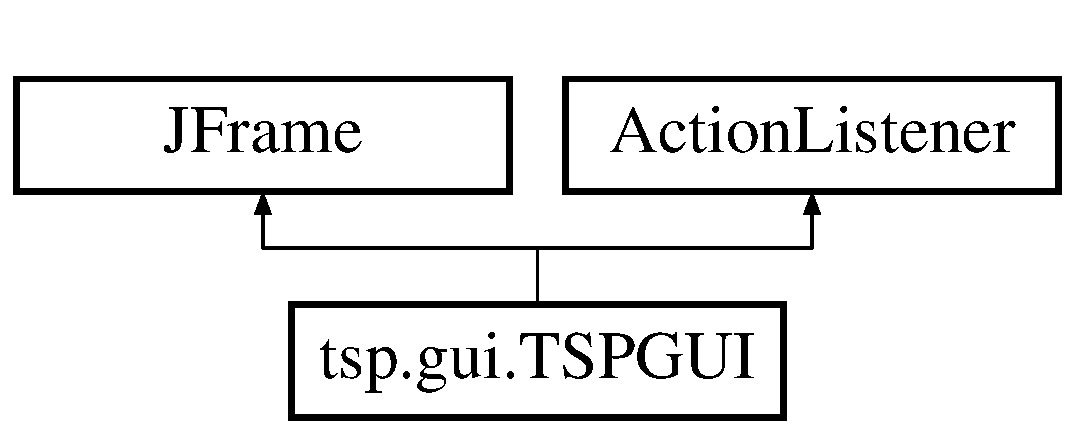
\includegraphics[height=2.000000cm]{classtsp_1_1gui_1_1_t_s_p_g_u_i}
\end{center}
\end{figure}
\subsection*{Public Member Functions}
\begin{DoxyCompactItemize}
\item 
\mbox{\Hypertarget{classtsp_1_1gui_1_1_t_s_p_g_u_i_ac73a45c3b122b01298636acd265895a9}\label{classtsp_1_1gui_1_1_t_s_p_g_u_i_ac73a45c3b122b01298636acd265895a9}} 
{\bfseries T\+S\+P\+G\+UI} (\mbox{\hyperlink{classtsp_1_1_solution}{Solution}} solution)
\item 
\mbox{\Hypertarget{classtsp_1_1gui_1_1_t_s_p_g_u_i_af3df3b3d93921721e1e35670bace851d}\label{classtsp_1_1gui_1_1_t_s_p_g_u_i_af3df3b3d93921721e1e35670bace851d}} 
void {\bfseries action\+Performed} (Action\+Event arg0)
\end{DoxyCompactItemize}
\subsection*{Static Public Member Functions}
\begin{DoxyCompactItemize}
\item 
\mbox{\Hypertarget{classtsp_1_1gui_1_1_t_s_p_g_u_i_abc3c3ac492a0a3fe6ae0d73c43381250}\label{classtsp_1_1gui_1_1_t_s_p_g_u_i_abc3c3ac492a0a3fe6ae0d73c43381250}} 
static double {\bfseries scale\+Coordinate} (double coordinate, double min, double max, double size, double offset)
\end{DoxyCompactItemize}


The documentation for this class was generated from the following file\+:\begin{DoxyCompactItemize}
\item 
src/tsp/gui/T\+S\+P\+G\+U\+I.\+java\end{DoxyCompactItemize}

\hypertarget{classtsp_1_1_t_s_p_solver}{}\section{tsp.\+T\+S\+P\+Solver Class Reference}
\label{classtsp_1_1_t_s_p_solver}\index{tsp.\+T\+S\+P\+Solver@{tsp.\+T\+S\+P\+Solver}}
\subsection*{Public Member Functions}
\begin{DoxyCompactItemize}
\item 
\mbox{\hyperlink{classtsp_1_1_t_s_p_solver_a0f6712f49bdce5b161b1bfd9f1112e91}{T\+S\+P\+Solver}} (\mbox{\hyperlink{classtsp_1_1_instance}{Instance}} instance, long time\+Limit)
\item 
void \mbox{\hyperlink{classtsp_1_1_t_s_p_solver_a9d4e4f4559a537b2af395fb8ab930906}{solve}} ()  throws Exception 	
\item 
\mbox{\hyperlink{classtsp_1_1_solution}{Solution}} \mbox{\hyperlink{classtsp_1_1_t_s_p_solver_a036aa2d65bd855929ff84886cb01f004}{get\+Solution}} ()
\item 
\mbox{\hyperlink{classtsp_1_1_instance}{Instance}} \mbox{\hyperlink{classtsp_1_1_t_s_p_solver_a981fdbf2b80722b258d99be5c22a2fab}{get\+Instance}} ()
\item 
long \mbox{\hyperlink{classtsp_1_1_t_s_p_solver_afa2c693c928addd2bee76ad2a4aed108}{get\+Time\+Limit}} ()
\item 
void \mbox{\hyperlink{classtsp_1_1_t_s_p_solver_af58c18bddbdd6d8fb67a8d1335913f14}{set\+Solution}} (\mbox{\hyperlink{classtsp_1_1_solution}{Solution}} solution)
\item 
void \mbox{\hyperlink{classtsp_1_1_t_s_p_solver_a962cd00f504347f89a69b2142dc9a400}{set\+Instance}} (\mbox{\hyperlink{classtsp_1_1_instance}{Instance}} instance)
\item 
void \mbox{\hyperlink{classtsp_1_1_t_s_p_solver_a13dec1ff9423995aa911859122b416a9}{set\+Time\+Limit}} (long time)
\end{DoxyCompactItemize}


\subsection{Detailed Description}
This class is the place where you should enter your code and from which you can create your own objects.

The method you must implement is \mbox{\hyperlink{classtsp_1_1_t_s_p_solver_a9d4e4f4559a537b2af395fb8ab930906}{solve()}}. This method is called by the programmer after loading the data.

The \mbox{\hyperlink{classtsp_1_1_t_s_p_solver}{T\+S\+P\+Solver}} object is created by the \mbox{\hyperlink{classtsp_1_1_main}{Main}} class. The other objects that are created in \mbox{\hyperlink{classtsp_1_1_main}{Main}} can be accessed through the following \mbox{\hyperlink{classtsp_1_1_t_s_p_solver}{T\+S\+P\+Solver}} attributes\+:
\begin{DoxyItemize}
\item \#m\+\_\+instance \+: the \mbox{\hyperlink{classtsp_1_1_instance}{Instance}} object which contains the problem data
\item \#m\+\_\+solution \+: the \mbox{\hyperlink{classtsp_1_1_solution}{Solution}} object to modify. This object will store the result of the program.
\item \#m\+\_\+time\+Limit \+: the maximum time limit (in seconds) given to the program.
\end{DoxyItemize}

\begin{DoxyAuthor}{Author}
Damien Prot, Fabien Lehuede, Axel Grimault 
\end{DoxyAuthor}
\begin{DoxyVersion}{Version}
2017 
\end{DoxyVersion}


\subsection{Constructor \& Destructor Documentation}
\mbox{\Hypertarget{classtsp_1_1_t_s_p_solver_a0f6712f49bdce5b161b1bfd9f1112e91}\label{classtsp_1_1_t_s_p_solver_a0f6712f49bdce5b161b1bfd9f1112e91}} 
\index{tsp\+::\+T\+S\+P\+Solver@{tsp\+::\+T\+S\+P\+Solver}!T\+S\+P\+Solver@{T\+S\+P\+Solver}}
\index{T\+S\+P\+Solver@{T\+S\+P\+Solver}!tsp\+::\+T\+S\+P\+Solver@{tsp\+::\+T\+S\+P\+Solver}}
\subsubsection{\texorpdfstring{T\+S\+P\+Solver()}{TSPSolver()}}
{\footnotesize\ttfamily tsp.\+T\+S\+P\+Solver.\+T\+S\+P\+Solver (\begin{DoxyParamCaption}\item[{\mbox{\hyperlink{classtsp_1_1_instance}{Instance}}}]{instance,  }\item[{long}]{time\+Limit }\end{DoxyParamCaption})\hspace{0.3cm}{\ttfamily [inline]}}

Creates an object of the class \mbox{\hyperlink{classtsp_1_1_solution}{Solution}} for the problem data loaded in \mbox{\hyperlink{classtsp_1_1_instance}{Instance}} 
\begin{DoxyParams}{Parameters}
{\em instance} & the instance of the problem \\
\hline
{\em time\+Limit} & the time limit in seconds \\
\hline
\end{DoxyParams}


\subsection{Member Function Documentation}
\mbox{\Hypertarget{classtsp_1_1_t_s_p_solver_a981fdbf2b80722b258d99be5c22a2fab}\label{classtsp_1_1_t_s_p_solver_a981fdbf2b80722b258d99be5c22a2fab}} 
\index{tsp\+::\+T\+S\+P\+Solver@{tsp\+::\+T\+S\+P\+Solver}!get\+Instance@{get\+Instance}}
\index{get\+Instance@{get\+Instance}!tsp\+::\+T\+S\+P\+Solver@{tsp\+::\+T\+S\+P\+Solver}}
\subsubsection{\texorpdfstring{get\+Instance()}{getInstance()}}
{\footnotesize\ttfamily \mbox{\hyperlink{classtsp_1_1_instance}{Instance}} tsp.\+T\+S\+P\+Solver.\+get\+Instance (\begin{DoxyParamCaption}{ }\end{DoxyParamCaption})\hspace{0.3cm}{\ttfamily [inline]}}

\begin{DoxyReturn}{Returns}
problem data 
\end{DoxyReturn}
\mbox{\Hypertarget{classtsp_1_1_t_s_p_solver_a036aa2d65bd855929ff84886cb01f004}\label{classtsp_1_1_t_s_p_solver_a036aa2d65bd855929ff84886cb01f004}} 
\index{tsp\+::\+T\+S\+P\+Solver@{tsp\+::\+T\+S\+P\+Solver}!get\+Solution@{get\+Solution}}
\index{get\+Solution@{get\+Solution}!tsp\+::\+T\+S\+P\+Solver@{tsp\+::\+T\+S\+P\+Solver}}
\subsubsection{\texorpdfstring{get\+Solution()}{getSolution()}}
{\footnotesize\ttfamily \mbox{\hyperlink{classtsp_1_1_solution}{Solution}} tsp.\+T\+S\+P\+Solver.\+get\+Solution (\begin{DoxyParamCaption}{ }\end{DoxyParamCaption})\hspace{0.3cm}{\ttfamily [inline]}}

\begin{DoxyReturn}{Returns}
the problem \mbox{\hyperlink{classtsp_1_1_solution}{Solution}} 
\end{DoxyReturn}
\mbox{\Hypertarget{classtsp_1_1_t_s_p_solver_afa2c693c928addd2bee76ad2a4aed108}\label{classtsp_1_1_t_s_p_solver_afa2c693c928addd2bee76ad2a4aed108}} 
\index{tsp\+::\+T\+S\+P\+Solver@{tsp\+::\+T\+S\+P\+Solver}!get\+Time\+Limit@{get\+Time\+Limit}}
\index{get\+Time\+Limit@{get\+Time\+Limit}!tsp\+::\+T\+S\+P\+Solver@{tsp\+::\+T\+S\+P\+Solver}}
\subsubsection{\texorpdfstring{get\+Time\+Limit()}{getTimeLimit()}}
{\footnotesize\ttfamily long tsp.\+T\+S\+P\+Solver.\+get\+Time\+Limit (\begin{DoxyParamCaption}{ }\end{DoxyParamCaption})\hspace{0.3cm}{\ttfamily [inline]}}

\begin{DoxyReturn}{Returns}
Time given to solve the problem 
\end{DoxyReturn}
\mbox{\Hypertarget{classtsp_1_1_t_s_p_solver_a962cd00f504347f89a69b2142dc9a400}\label{classtsp_1_1_t_s_p_solver_a962cd00f504347f89a69b2142dc9a400}} 
\index{tsp\+::\+T\+S\+P\+Solver@{tsp\+::\+T\+S\+P\+Solver}!set\+Instance@{set\+Instance}}
\index{set\+Instance@{set\+Instance}!tsp\+::\+T\+S\+P\+Solver@{tsp\+::\+T\+S\+P\+Solver}}
\subsubsection{\texorpdfstring{set\+Instance()}{setInstance()}}
{\footnotesize\ttfamily void tsp.\+T\+S\+P\+Solver.\+set\+Instance (\begin{DoxyParamCaption}\item[{\mbox{\hyperlink{classtsp_1_1_instance}{Instance}}}]{instance }\end{DoxyParamCaption})\hspace{0.3cm}{\ttfamily [inline]}}

Sets the problem data 
\begin{DoxyParams}{Parameters}
{\em instance} & the \mbox{\hyperlink{classtsp_1_1_instance}{Instance}} object which contains the data. \\
\hline
\end{DoxyParams}
\mbox{\Hypertarget{classtsp_1_1_t_s_p_solver_af58c18bddbdd6d8fb67a8d1335913f14}\label{classtsp_1_1_t_s_p_solver_af58c18bddbdd6d8fb67a8d1335913f14}} 
\index{tsp\+::\+T\+S\+P\+Solver@{tsp\+::\+T\+S\+P\+Solver}!set\+Solution@{set\+Solution}}
\index{set\+Solution@{set\+Solution}!tsp\+::\+T\+S\+P\+Solver@{tsp\+::\+T\+S\+P\+Solver}}
\subsubsection{\texorpdfstring{set\+Solution()}{setSolution()}}
{\footnotesize\ttfamily void tsp.\+T\+S\+P\+Solver.\+set\+Solution (\begin{DoxyParamCaption}\item[{\mbox{\hyperlink{classtsp_1_1_solution}{Solution}}}]{solution }\end{DoxyParamCaption})\hspace{0.3cm}{\ttfamily [inline]}}

Initializes the problem solution with a new \mbox{\hyperlink{classtsp_1_1_solution}{Solution}} object (the old one will be deleted). 
\begin{DoxyParams}{Parameters}
{\em solution} & \+: new solution \\
\hline
\end{DoxyParams}
\mbox{\Hypertarget{classtsp_1_1_t_s_p_solver_a13dec1ff9423995aa911859122b416a9}\label{classtsp_1_1_t_s_p_solver_a13dec1ff9423995aa911859122b416a9}} 
\index{tsp\+::\+T\+S\+P\+Solver@{tsp\+::\+T\+S\+P\+Solver}!set\+Time\+Limit@{set\+Time\+Limit}}
\index{set\+Time\+Limit@{set\+Time\+Limit}!tsp\+::\+T\+S\+P\+Solver@{tsp\+::\+T\+S\+P\+Solver}}
\subsubsection{\texorpdfstring{set\+Time\+Limit()}{setTimeLimit()}}
{\footnotesize\ttfamily void tsp.\+T\+S\+P\+Solver.\+set\+Time\+Limit (\begin{DoxyParamCaption}\item[{long}]{time }\end{DoxyParamCaption})\hspace{0.3cm}{\ttfamily [inline]}}

Sets the time limit (in seconds). 
\begin{DoxyParams}{Parameters}
{\em time} & time given to solve the problem \\
\hline
\end{DoxyParams}
\mbox{\Hypertarget{classtsp_1_1_t_s_p_solver_a9d4e4f4559a537b2af395fb8ab930906}\label{classtsp_1_1_t_s_p_solver_a9d4e4f4559a537b2af395fb8ab930906}} 
\index{tsp\+::\+T\+S\+P\+Solver@{tsp\+::\+T\+S\+P\+Solver}!solve@{solve}}
\index{solve@{solve}!tsp\+::\+T\+S\+P\+Solver@{tsp\+::\+T\+S\+P\+Solver}}
\subsubsection{\texorpdfstring{solve()}{solve()}}
{\footnotesize\ttfamily void tsp.\+T\+S\+P\+Solver.\+solve (\begin{DoxyParamCaption}{ }\end{DoxyParamCaption}) throws Exception\hspace{0.3cm}{\ttfamily [inline]}}

{\bfseries T\+O\+DO} Modify this method to solve the problem.

Do not print text on the standard output (eg. using {\ttfamily System.\+out.\+print()} or {\ttfamily System.\+out.\+println()}). This output is dedicated to the result analyzer that will be used to evaluate your code on multiple instances.

You can print using the error output ({\ttfamily System.\+err.\+print()} or {\ttfamily System.\+err.\+println()}).

When your algorithm terminates, make sure the attribute \#m\+\_\+solution in this class points to the solution you want to return.

You have to make sure that your algorithm does not take more time than the time limit \#m\+\_\+time\+Limit.


\begin{DoxyExceptions}{Exceptions}
{\em Exception} & may return some error, in particular if some vertices index are wrong. \\
\hline
\end{DoxyExceptions}


The documentation for this class was generated from the following file\+:\begin{DoxyCompactItemize}
\item 
src/tsp/T\+S\+P\+Solver.\+java\end{DoxyCompactItemize}

%--- End generated contents ---

% Index
\backmatter
\newpage
\phantomsection
\clearemptydoublepage
\addcontentsline{toc}{chapter}{Index}
\printindex

\end{document}
